\documentclass[MASTER.tex]{subfiles}
\begin{document}
	\chapter{Limits of Agreement}
	
% % JOBS
% % Mantha Et Al
% % Barnhart's Paper	
%----------------------------------------------------------------------------%
\section{Limits of Agreement}
% introduces
A third element of the Bland-Altman methodology, an interval known
as `limits of agreement' is introduced in \citet*{BA86}
(sometimes referred to in literature as 95\% limits of agreement). Bland and Altman proposed a pair of Limits of agreement. These
limits are intended to demonstrate the range in which 95\% of the
sample data should lie. The Limits of agreement centre on the
average difference line and are 1.96 times the standard deviation
above and below the average difference line.
Limits of agreement are used to assess whether the two methods of
measurement can be used interchangeably. \citet{BA86} refer to
this as the `equivalence' of two measurement methods. The specific purpose of the limits of
agreement must be
established clearly. \citet*{BA95} comment that the limits of agreement `\textit{how
far apart measurements by the two methods were likely to be for
most individuals}', a definition echoed in their 1999 paper:

\begin{quote}"We can then say that nearly all pairs
	of measurements by the two methods will be closer together than
	these extreme values, which we call 95\% limits of agreement.
	These values define the range within which most differences
	between measurements by the two methods will lie."
\end{quote}


The limits of agreement (LoA) are computed by the following
formula:
\[
LoA = \bar{d} \pm 1.96 s_{d}
\]
with $\bar{d}$ as the estimate of the inter method bias, $s_{d}$
as the standard deviation of the differences and 1.96 is the 95\%
quantile for the standard normal distribution. (Some descriptions of the
Bland-Altman plot use 2 standard deviations instead
for simplicity.)

The limits of agreement methodology assumes a constant level of bias throughout the range of measurements. Importantly the authors recommend prior determination of what would and would constitute acceptable
agreement, and that sample sizes should be predetermined to give an accurate conclusion. 

\begin{quote}
	``How far apart measurements can be without causing difficulties
	will be a question of judgment. Ideally, it should be defined in
	advance to help in the interpretation of the method comparison and
	to choose the sample size \citep{BA86}".
\end{quote}

However \citet{mantha} highlights inadequacies in the correct application of limits of agreement, resulting in contradictory estimates for limits of agreement in various papers.

For the Grubbs `F vs C' comparison, these limits
of agreement are calculated as -0.132 for the upper bound, and
-1.08 for the lower bound. Figure ~\ref{GrubbsBAplot-noLOA} shows the resultant
Bland-Altman plot, with the limits of agreement shown in dashed
lines.


\begin{figure}[h!]
	\begin{center}
		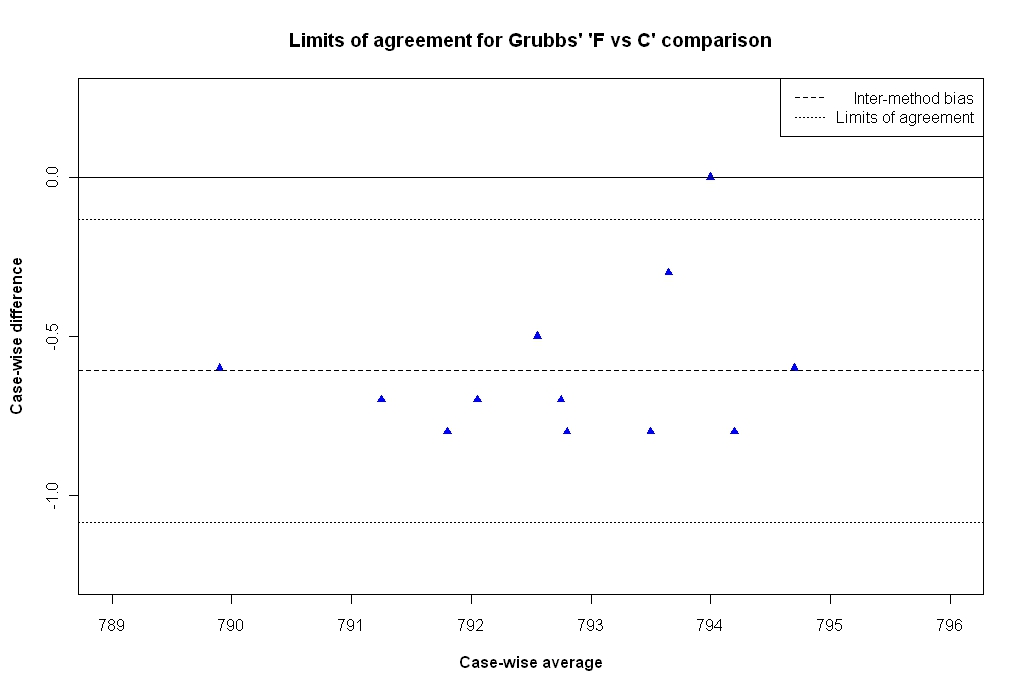
\includegraphics[width=125mm]{GrubbsBAplot-LOA.jpeg}
		\caption{Bland-Altman plot with limits of agreement}\label{GrubbsBAplot-noLOA}
	\end{center}
\end{figure}
\newpage

%But as \citet*{BA86} point out this may not be the case. Variants of the limits of agreement that overcome this
% problem shall be introduced in due course.

%========================================================== %
\newpage
\section{Interpretation of Limits Of Agreement}

How this relates the overall population is unclear. It seems that it depends on an expert to decide whether or not the range of differences is acceptable. 

If one method is sometimes higher, and sometimes the other method is higher, the average of the differences will be close to zero. If it is not close to zero, this indicates that the two assay methods are producing different results systematically.

\subsection{Formal Definition of Limits of Agreement}
\citet{BA99} note the similarity of limits of agreement to
confidence intervals, but are clear that they are not the same thing. Interestingly, they describe the limits as `\textit{being like a reference interval}'.

Limits of agreement have very similar construction to Shewhart control limits. The Shewhart chart is a well known graphical
methodology used in statistical process control. Consequently there is potential for misinterpreting the limits of agreement as if equivalent to Shewhart control limits. Importantly the
parameters used to determine the Shewhart limits are not based on any sample used for an analysis, but
on the process's historical values, a key difference with
Bland-Altman limits of agreement.

\citet{BXC2008} regards the limits of agreement as a prediction interval for the difference between future measurements with the two methods on a new individual, but states that it does not fit
the formal definition of a prediction interval, since the definition does not consider the errors in estimation of the
parameters. Prediction intervals, which are often used in regression analysis, are estimates of an interval in which future
observations will fall, with a certain probability, given what has already been observed. \citet{BXC2008} offers an alternative formulation, a $95\%$ prediction interval for the difference
\[
\bar{d} \pm t_{(0.975, n-1)}s_{d} \sqrt{1+\frac{1}{n}}
\]

\noindent where $n$ is the number of subjects. Carstensen is
careful to consider the effect of the sample size on the interval
width, adding that only for 61 or more subjects is there a
quantile less than 2.

Various other interpretations as to how limits of agreement should properly be defined. \citet{luiz} offers an alternative description of limits of
agreement, this time as tolerance limits. A tolerance interval for
a measured quantity is the interval in which a specified fraction
of the population's values lie, with a specified level of
confidence. \citet{Barnhart} describes them as a probability
interval, and offers a clear description of how they should be
used; `\textit{if the absolute limit is less than an acceptable difference
$d_{0}$, then the agreement between the two methods is deemed
satisfactory}'.

The prevalence of contradictory definitions of what limits of agreement strictly are will inevitably attenuate the poor standard of reporting using limits of agreement, as discussed by \citet{mantha}.

%At least 100 historical
%values must be used to determine the acceptable value (i.e the
%process mean) and the process standard deviation. The principle
%that the mean and variance of a large sample of a homogeneous
%population is a close approximation of the population's mean and
%variance justifies this.

%\begin{figure}[h!]
%\begin{center}
%  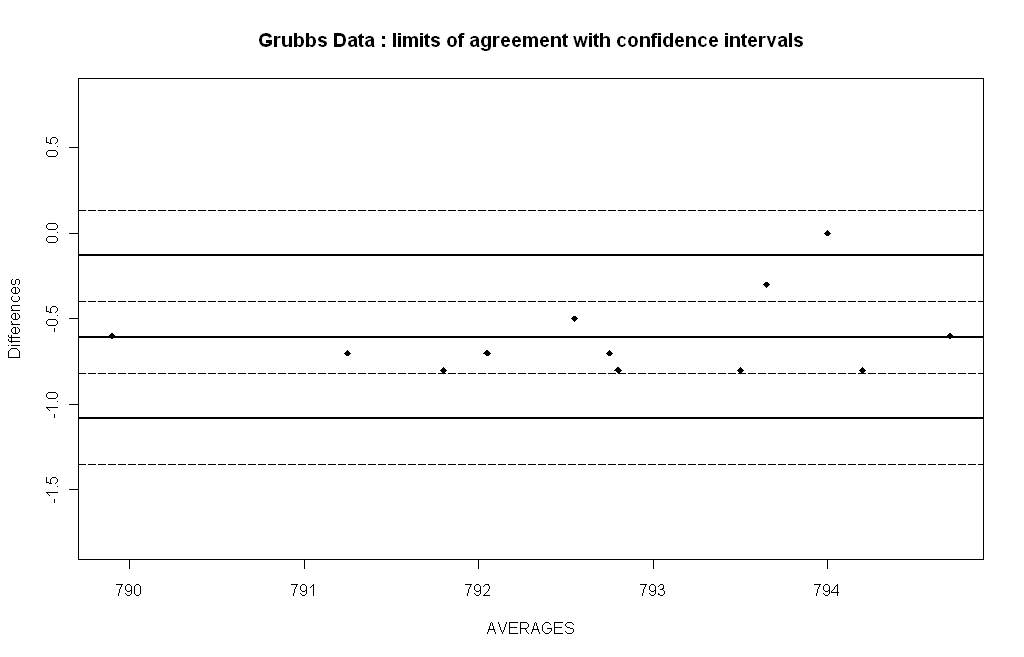
\includegraphics[width=125mm]{GrubbsLOAwCIs.jpeg}
%  \caption{Limits of agreement with confidence intervals}\label{LOAwCIs}
%\end{center}
%\end{figure}









\section{Limits of Agreement for Replicate Measurements}

Computing limits of agreement features prominently in many method comparison studies since the publication of \citet{BA86}.
\citet{BA99} addresses the issue of computing LoAs in the presence of replicate measurements, suggesting several computationally simple approaches. When repeated measures data are available, it is desirable to use
all the data to compare the two methods. However, the original Bland-Altman method was developed for two sets of measurements done on one occasion, and so this approach is not suitable for replicate measures data. However, as a naive analysis, it may be used to explore the data because of the simplicity of the method.
In addition to \citet{BA99}, \citet{BXC2008} computes the limits of agreement to the case with replicate measurements by using LME models, an approach that will be discussed in due course.

\subsubsection{Precision of Limits of Agreement}
The limits of agreement are estimates derived from the sample
studied, and will differ from values relevant to the whole
population. A different sample would give different limits of
agreement. \citet*{BA86} advance a formulation for confidence
intervals of the inter-method bias and the limits of agreement.
These calculations employ quantiles of the `t' distribution with
$n -1$ degrees of freedom.

%This page also shows the standard deviation (SD) of the
%differences between the two assay methods. The SD value is used to
%calculate the limits of agreement, computed as the mean bias plus
%or minus 1.96 times its SD.
%----------------------------------------------------------------------------%
\subsection{Appropriate Use of Limits of Agreement}
Importantly \citet{BA99} makes the following point:
\begin{quote}These estimates are meaningful only if we can assume
	bias and variability are uniform throughout the range of
	measurement, assumptions which can be checked graphically.
\end{quote}

The import of this statement is that, should the Bland-Altman plot indicate that these assumptions are not met, then their entire methodology, as posited thus far, is inappropriate for use in a method comparison study. Again, in the context of potential outlier in the Grubbs data (figure 1.2), this raises the question on how to correctly continue.
%
%Carstensen attends to the issue of repeated data, using the
%expression replicate to express a repeated measurement on a
%subject by the same methods. Carstensen formulates the data as
%follows Repeated measurement - Arrangement of data into groups,
%based on the series of results of each subject.


	%At least 100 historical
	%values must be used to determine the acceptable value (i.e the
	%process mean) and the process standard deviation. The principle
	%that the mean and variance of a large sample of a homogeneous
	%population is a close approximation of the population's mean and
	%variance justifies this.
	
	%\begin{figure}[h!]
	%\begin{center}
	%  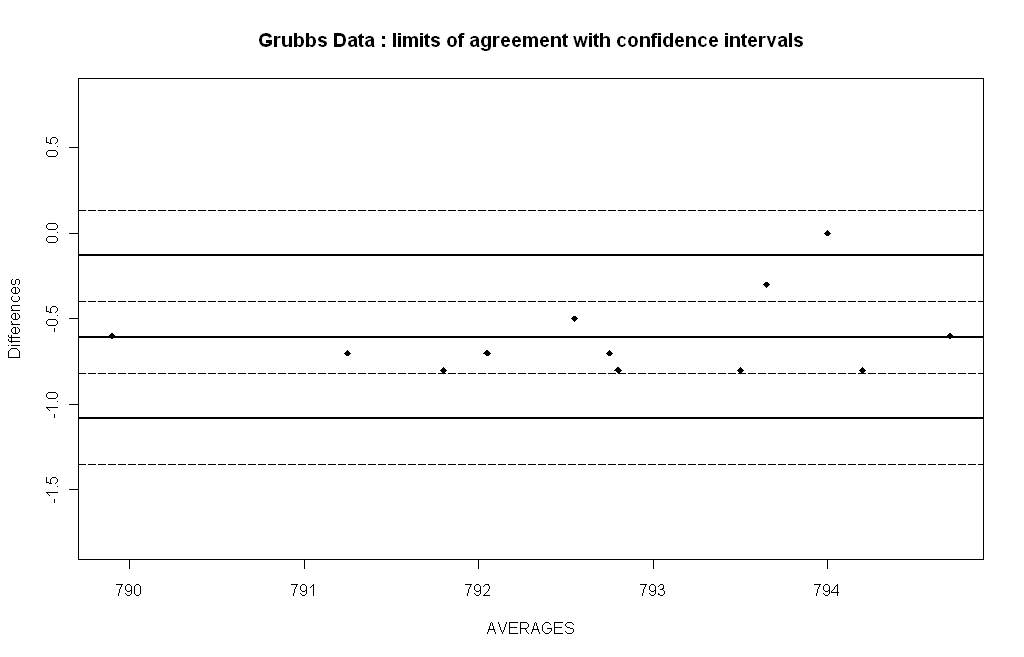
\includegraphics[width=125mm]{GrubbsLOAwCIs.jpeg}
	%  \caption{Limits of agreement with confidence intervals}\label{LOAwCIs}
	%\end{center}
	%\end{figure}
	
	
	
	\newpage
	%---------------------------------------------%
	\section{Coefficient of Repeatability}
	\subsection{Repeatability}
	As mentioned previously, \citet{Barnhart} emphasizes the importance of repeatability as part of an overall method comparison study. The coefficient of repeatability was proposed by \citet{BA99}, and is referenced in subsequent papers, such as \citet{BXC2008}. The coefficient of repeatability is a measure of how well a
	measurement method agrees with itself over replicate measurements
	\citep{BA99}. The coefficient of repeatability is a measure of how well a
	measurement method agrees with itself over replicate measurements
	\citep{BA99}. Once the the standard deviations of the differences between the two measurements (in some texts called the residual standard deviation or within-item variability) $sigma_m$ is determined, the
	computation of the coefficients of repeatability for both methods
	is straightforward. The coefficient is calculated from the (in some texts called the residual standard deviation) as  $1.96 \times \sqrt{2} \times \sigma_m$ = $2.83 \sigma_m$).
	
	

	%------------------------------------------------------------------------------%
	
	\subsection{Repeatability coefficient}
	\citet{BA99} introduces the repeatability coefficient for a method, which is defined as the upper limits of a prediction interval for the absolute difference between two measurements by the same
	method on the same item under identical circumstances \citep{BXC2008}.
	
	$\sigma^2_{x}$ is the within-subject variance of method $x$. The repeatability coefficient is $2.77 \sigma_{x}$ (i.e. $1.96 \times \sqrt{2} \sigma_{x}$). For $95\%$ of subjects, two replicated measurement by the same method will be within this repeatability coefficient.
	

	
	
	
%	\bibliography{DB-txfrbib}
\end{document}